
\chapter{le \og CPD\fg: Conception de protéine par ordinateur}
\label{chap:CPD}

L'ingénierie des protéines est l'ensemble des techniques qui ont pour objet de modifier la fonction, ou la structure d'une protéine en modifiant sa séquence d'acide aminés.Les objectifs sont d'augmenter la stabilités des protéines, à modifier des fonctionnements enzymatiques ou encore à ajouter une conformation altéernative à une protéine.
Dans ce domaine, existe la mutagénèse dirigée dans laquelle sont une première étape est l'identification des mutations interessantes pour l'objectif fixé, puis des méthodes de génie génétique sont utilisées pour produire les mutants dont les propriétés souhaitées pourront être vérifiées a posteriori.Une deuxième approche est l'évolution dirigée, dans laquelle un ensemble de mutation aléatoire est effectué sur une séquence de protéine d'intérêt et toutes les séquences ainsi produites sont testé afin de trouver la caractéristique atendue.La selection de fait alors, comme pour l'evolution naturelle dont elle reprend les mécanismes, sur les séquences positives aux tests.


   \begin{figure}[t]
     \centering
     \begin{tabular}{c}
       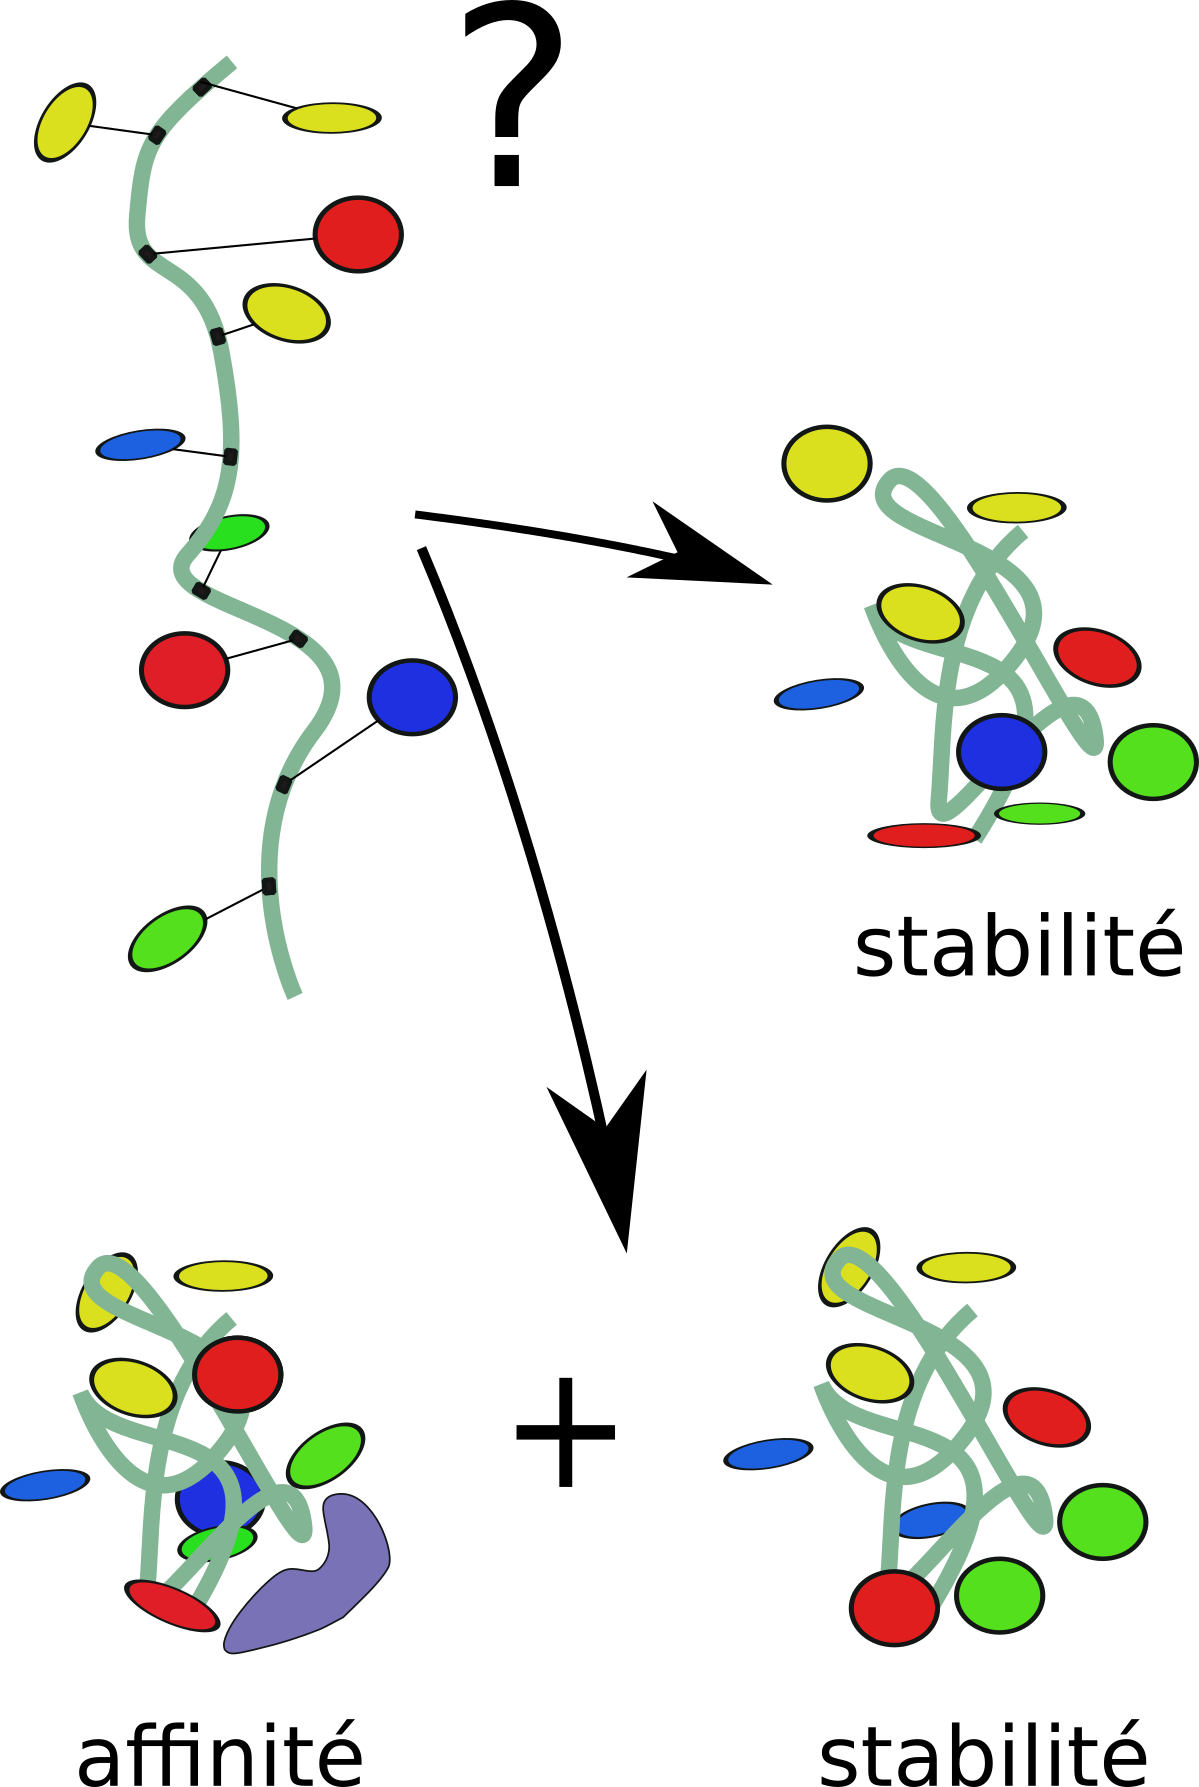
\includegraphics[width=6cm]{graphe/proteus/CPD.png} &
     \end{tabular}
     
     \caption{Le CPD dans proteus}
\label{graph:struct_Phy}
   \end{figure}


Un autre approche est d'utiliser de la capacité de calculs des ordinateurs, avec l'apparition des méthodes d'ingénierie des protéines \og in silico\fg.L'unes d'elles, le \og Computational Protein Design\fg ou CPD conciste à déterminer les séquences d'acides aminés compatibles avec une structure protéique donnée, on parle également du problème inverse du repliement. Ce qui implique la connaissance de la structure dans l'espace 3D de la protéine.Cette méthode comporte trois élèments principaux.

\begin{enumerate}
\item la determination d'un espace de conformation de la protéine
  C'est sur elle que repose la prédiction de structure des séquences considérées.Elle doit être capable de de representer une ou un petit nombre de conformation de la chaîne principale du polypeptide et tout un ensemble dede poistionnemnent de la chaîne latérale de chacun des résidues.
\item Un fonction d'énergie, qui permet d'évaluer la pertinence des conformations 
\item Un algorithme d'exploration de l'espace de conformation qui permet grâce à la fonction d'énergie d'échantilloner les séquences favorables.
  
\end{enumerate}

Dans ce chapitre, nous aborterons le problème de la modélisation des protéines et de leur espace de conformation et de l'espace onformation-séquence. Puis, nous verrons les fonctions d'énergies classiques pour une conformation.Ensuite, sera detaile , les approches possibles pour la modélisation du solvant. Plusieurs algorithmes d'explorations de l'ensembles des conformations serrons vue. Les principaux programme CPD seront énumèrés. Et enfin, nous présenterons quelques applications du CPD.   


\section{l'espace des séquences-conformations}

L'ensemble des cas possibles à prendre en compte, peut se concevoir comme un choix d'un $S$ séquence de longueur $N$  et pour $S$ la determination d'un conformation $C$. Ainsi l'espace d'état est celui de l'ensemble de couples. $(S,C)$ pour $N$ donnée. Dans toute la suite on appelle une séquence-conformation un élément de cet ensemble de couples.   

L'ensemble des séquences de $N$  acides aminés se concoit sans diffcultés. En revanche,l'ensemble des conformations d'une chaîne polypeptidique doit être défini explicitement.

\subsection{l'état replié }
La mécanique moléculaire propose d'utiliser les représentations de la mécanique classique aux molécules.Les atomes sont représent forme de sphère.Ces objects sont alors considérer être plonger dans un espace 3D euclidien.
La protéine dans un milieu aqueux est fléxible et en permanence en mouvement.C'est en particulier le cas pour les chaînes latérales ou pour les boucles flexibles. L'espace des d'états d'une protéine, dans le cadre de la mécanique moléculaire est alors constitue un vaste espace continue de conformation possibles. D'autrepart si un polypeptide a un nombre $n$ de résidus compris entre $50$ et $100$ , et que chacunes des $n$ positions de la chaîne peut muter $20$ types differents d'acide aminés, le nombre de polypeptide à considérer est égale à  $n^{20}$.Il est donc nécessaire de réduire la taille de l'espace des conformations à prendre en compte.Pour cela, Ponder & Richards [1987] propose une approche en deux points:
\begin{enumerate}
\item Le squelette de la protéine est fixé.
\item Les conformations des chaînes latérales sont reduites à un ensemble fini de positionnenent dans l'espace 3D.
\end{enumerate}  
Ensuite, des variations sur ce principe ont étés introduites, avec notament l'introductoin de la prise en compte de la mobilité de la chaîne principale dans un ensemble discret ou continu d'état.L'approche qui consiste à générer un ensemble de squelettes et a faire des calculs CPD pour l'ensemble a été utilisé par [137]. 
Nous présentons maintenant, la modélisation des chaînes latérales et celle du backbone.

\subsubsection{les chaînes latérales}

les travaux de Finkelstein et Ptitsyn [77],Janin et al [78] ainsi que Ponder et Rischars [87] ont établie que la chaîne latérales des résidues, sur un ensemble de protéines, adope de facon préférentiel un petit ensemble de conformation (fig \ref{..}). Janin introduit alors le terme de \og rotamère\fg pour désigner ces conformations. Il est alors possible reduite l'espace continue des conformations des acides aminés à cette ensemble discret de rotamères.la plupart des méthodes de CPD utilisent cette discrétisation.Beaucoup de librairies de rotamères ont été proposées dans la litérarure scientifique. la plupart sont indépendantes du backbone. Mais il existe également des librairies qui dépendent du squelette de la protéine voir [147,148].Le nombre de structures de protéine utilisé est variable , La librairie de Tufféry utlise 53 structures. 

\subsubsection{Le squelette}
Partant du fait que les positionnements des chaînes latérales ne modifie que faiblement la structure adoptée par le backbone,la chaîne principale de la protéine est fixé dans beaucoup de programme CPD. Le problème de la prédiction de struture est alors ramener à celui du placement des chaînes latérale sur ce squelette. De part la configuration particulière de la proline avec le backbone de type est traité a part. Cette approche a obtenue de nombreux succès , voir \ref{...}.
Cependant, cette approximation peu avoir des consequences importantes.Un type d'acide aminé considéré comme défavorable peut devenir favorable avec une petite adapation du backbone et il a été établie que quelques mouvements de squelettes peuvent faire varié significativement l'énergie de la conformation (Desjarlais et Handel [1999]).
En réponse à ce problème, [137] propose de générer un ensemble de squelettes et de faire du CPD pour chacun des exemplaires obtenus. Une autre approche consiste à donner une certaine liberté aux angles $\Phi$ , $\Psi$ en introudisant des variations aliéatoires sur ceux-ci (Desjarlais et Handel)[141].
Puis raissament, De Dantas et al [2007] font des simulations avec une minimisation après chaque mouvement de chaîne latérale.Kuhlman et al [2003] optimisent alternativement la structure du squelette et la séquence d'acide aminés.Enfin, citont l'utilisation du classes particulier de mouvement des squelettes protéiques appelé \og backrub \fg. Ce sont des mouvements naturels du backbone mis en évidence par David et al [2006], à partir de structures cristallographiques. Ces mouvenent consiste en des déplacement de l'ensemble $C_{\alpha}-C_{\beta}$ à une position $i$ donnée de la chaîne, sans déplacement des carbones $C_{\alpha_{i+1}}$ et $C_{\alpha_{i-1}}$ . Ces mouvements backrub ont permis à Georgiev et al [2008] et Smith et Kortemme [2008] d'améliorer la qualité des prédiction des mutants par rapport à des simllutations à squelette rigide.

\subsection{l'état deplié }
Lorsque la stabilité d'une protéine est évalué par une variation de l'énergie libre entre son état déplié et son état replié, il faut connaître l'énergie de l'état déplié.mais cet état est déstructré et ne correspond pas à une conformation unique; la modélisation hexaustive est difficile. Une approche simple consite à représenter cet état par une chaîne étendue; un résidu de la protéine est en interaction principalement avec le solvant et avec le backbone.Ainsi l'énergie libre de l'état déplié dépend de la séquence uniquement par la composition en acide aminés de celle-ci.En pratique, on peut utiliser pour chaque type d'acide aminé X de la protéine  un tripeptide ALA--X--ALA , et on identifie son exposition au solvant à celle de X dans l'état déplié [152] Dahiyat & Mayo [1996]. On en déduit une énergie définie par type X que l'on somme pour l'énergie de la protéine dépliée. 

\section{l'énegie de conformation}

La fonction d'énergie ou fonction de score,  de conformation permet d'évaluer la stabilité ( ou une affinité avec un ligand) de chaque conformation de la protéine. Cette fonction doit être capable de prendre en compte les détails des interactions entre les atomes de la protéine, les effets de l'environnement aqueux  dans lequel elle se trouve et en même temps être suffisament rapide pour évaluer en un temps raisonnable une partie la plus significative possible de l'espace des conformations.Une classe importante est constitué des fonctions d'énergie basée sur la mécanique moléculaire.

\subsection{La mécanique moléculaire}
\label{sub:mecamol}
La mécanique moléculaire représente les atomes comme des particules sphériques ayant une charge électrique nette fixe et chaque liaison est modélisé par ressort.
Cette mécanique consiste à intégrer les équations du mouvement de la mécanique classique dans un champ de force propre aux molécules étudiés.Ce champ de force décrit les interactions inter-atomiques du point de vue énergétique et est invariant au cours d'une simulation.
Dans la suite, nous appelons $E_{MM}$ l'énergie qui dérive d'un tel champs de force.

Il existe beaucoup de champs de force à la disposition des simulateurs voici les quatre principaux optimisés pour les protéines:

\begin{enumerate}
\item AMBER: Assisted Model Building with Energy Refinement [106]
\item CHARMM: Chemistry at HARvard Molecular Mechanics [105]
\item OPLS: Optimized Potential for Liquid Simulations [107]
\item GROMOS:GROningen MOlecular Simulation [108]
\end{enumerate}

L'énergie d'une conformation se défini alors comme la somme de l'énergie $E_{MM}$  et de l'énergie de solvatation:

\begin{equation}
  E = E_{MM} + E_{solv}
\end{equation}

Le terme $E_{MM}$ se décompose en :

\begin{equation}
  E_{MM} = E_{liées} + E_{non_liées}
\end{equation}

avec $E_{lié}$ l'énergie d'interactions des atomes éloignés d'au plus deux liaisons covalentes et $E_{inbond}$  l'énergie des autres interactions.Détaillons ces deux énergies

\subsection{Les interactions liées }

L'énergie d'interaction lié comprend un terme d'élongation des liaisons,un terme de déformation des angles, de rotation des angles dièdres, de torsions, des interactions de Van der Waals, enfin un terme électrostatique de Coulomb.


\begin{equation}
  E_{liées} = E_{liaison} + E_{angle} +E_{dièdre} + E_{impropre}
\end{equation}


\begin{enumerate}
\item L'énergie de déformations des liaisons $E_{liaison}$ s'exprime de la façon suivante:
  \begin{equation}
    E_{liaison} = \frac{1}{2} \sum_{i=1}^{n} k_{i} (r_i - r^o_i)^2
  \end{equation}
  avec l'ensemble des liaisons indexé par $i$, $k_{i}$ la force du ressort, $r_{i}$ la longeur de la liaison et $r^0_i$ la longeur optimale.
\item L'énergie de déformation des angles $E_{angl}$ est s'exprime:
    \begin{equation}
      E{angl} =\frac{1}{2} \sum_{ij}k_{\theta,ij}(\theta_{ij} - \theta_{ij}^0)^2
    \end{equation}
  avec $\theta_{ij}$ l'angle entre les liasons i et j, $\theta_{ij}^0$ l'angle optimal et $k_{\theta,ij}$ la force du ressort.
\item L'énergie de déformation des angles dièdres $E_{dièdre}$ est décrite par:
\begin{equation}
E_{dihe} = \frac{1}{2}\sum_{i} A_{i,n}[ 1 + cos(n\Phi_i - \Phi_0\)]
\end{equation}
  où n est périodicité de la rotation,$A_{i,n}$ est la constante de torsion,$\Phi_i$ l'angle dièdre, c'est à dire pour 4 atomes $a_1$,$a_2$,$a_3$ et $a_4$, reliées par 3 liaisons $a_1-a_2,a_2-a_3$ et$ a_3-a_4$, l'angle formé par les projetés de $a_1-a_2$ et $a_3-a_4$ sur un plan perpendiculaire à $a_2-a_3$. $\Phi^0$ est la phase.
\item L'énergie de déformation des angles impropres $E_{impr}$ exprime la déformation d'un  ensemble  de 4 atomes  par rapport à une conformation planaire ou tétraédrique.Pour un atome $a_1$ relié à 3 atomes $a_1$,$a_2$ et $a_3$,elle a la forme:
  \begin{equation}
    E_{impr}= \frac{1}{2}A(\Phi - \Phi^0)^2
  \end{equation}
  Ici, $A$ est la constante de force et $\Phi$ représente l'angle entre le plan ($a_1$,$a_2$,$a_3$) et la liason ($a_1$,$a_2$).
\end{enumerate}  

voir la figure \ref{...} pour une représentation visuelle.

\subsection{Les interactions non liées}
Les interactions non liées sont les interactions des atomes séparés par plus de trois liaisons covalentes ou qui appartiennent à des molécules différentes.les interactions sont caractérisées par deux les termes suivants:
\begin{equation}
E{non liées} = E{elec} + E{vdw}  
\end{equation}


\begin{enumerate}
  \label{VdW}
\item L'énergie $E_{elec}$ pour l'énergie électrostatique est donnée par un potentiel de Coulomb de la forme:
  \begin{equation}
    E{elec}=\frac{q_i.q_j}{\epsilon r_{ij}}
  \end{equation}
  avec $q_i$ et $q_j$ qui représentent les charges respectives des atomes $i$ et $j$ et $r_{ij}$ représente la distance netre les atomes $i$ et $j$ , enfin $\epsilon$ et la constante diélectrique du milieu.
\item L'énergie  $E_{vdW}$ pour l'énergie de Van der Waals, elle est du aux interactions électriques de faible intensité entre deux atomes, du au répartition des charges éléctriques.Cette énergie rassemble des effets des forces de Keesom,Delye,London et Pauli.Le potentiel de Lennard-Jones est l'approximation classique suivante de cette énergie:
  \begin{equation}
  E_{vdw} = \sum_{i<j}D_0 [(\frac{r_0}{r_{ij}})^12 - (\frac{r_0}{r_{ij}})^6]  
  \end{equation}
avec $D_0$ et $r_0$ des constantes, $r_{ij}$ la distance entre l'atome $i$ et l'atome $j$. Le premier terme est répulsif à courte distance, ce que permet d'éviter l'encombrement stérique entre $i$ et $j$ . le second terme domine à grande distance et est attractif. 
  
\end{enumerate}


\subsection{d'autres approches}

Même si la mécanique moléculaire prédomine dans le monde du CPD , il existe d'autres approches.Mayo [2006] utilise une fonction empirique pour la modélisation des liaisons hydrogènes, d'une focntion d'énergie coulombienne qui contient un $\epsilon$ qui varie en fonction de la distance interatomique.Il existe des fonctions d'énergie  conportant des élements relevant de statisque sur les protéines. Il existe encore des fonctions d'énergie à gros grains notament dans la modélisation des forces de Van der Walls utiles pour les applications d'interactions protéine-protéine.

\section{Modélisation du solvant}
Les protéines sont étudiées dans un solvant aqueux.C'est à dire que la solution qui est considérée dans les calculs est une mélange dans laquelle l'eau est présente en quantité largement plus importante que la quantité de protéine (les solutés). Bien qu'il existe d'autres type de solvant, ils ne sont pas abordé ici. Les interactions entre solutés et le solvant jouent un rôle clé dans le structure de la protéine mais également dans sa fonction. La modélisation du solvant est alors un point capital dans le CPD.

Une molécule d'eau a une charge électrique nette nulle.Mais il existe une dissymétrie du nuage électronique: Les électrons se situent de façon preferenciel au voisinnafe de l'atome d'oxygène par rapport au voisinnage des noyaux d'hydrogènes.
On dit que la molécule est polaire, et cette polarisation peut être approximée par un moment dipolaire.Cette polarité facilite la formation de liaisons hydrogènes entre molécules d'eau et avec tous autres groupes polaires. 
Ainsi, l'eau a état liquide possède beaucoup de liaisons hydrogènes. Lorsqu'une protéine est solvaté, les molécules du solvent se place de tel façon que le nombre de liaisons hydrogène soit maximal.Les molécules de la première couche de solvatation forme alors des liaisons avec les groupes polaires de la protéines ou pour les groupes non-polaires s'oriente pour former des liasons avec d'autres molécules d'eau. Cette reorganisation de la structure moléculaire de d'eau a trois conséquences importantes:

\begin{itemize}
\item une diminution de l'entropie au voisinnage de la protéine 
\item la creation de polarisation à la surface du soluté
\item  l'eau crée une couche de charges partielles opposées à celles de la protéine qui atténue le champ de celle-ci. ce phénomène s'appelle l'écrantage.
\end{itemize}
  
Il a été démontré d'une protéine et une molécule d'eau peuvent intéragir de façon non négligable jusqu'à une distance de 15 angstroms.Cela implique que pour solvaté correctement une protéine il faut prendre au compte l'effet de plusieurs milliers d'atomes du solvant.
De nombreuses méthodes ont été développées tentant de faire face à la difficilté que cela représente.
La connaissance des positions et les vitesses de toutes les molécules d'eau nécessaire dans le cadre de la mécanique moléculaire, apparaît alors comme une gageure. Des approches moins fines vont devoir être utilisées. 

\subsection{modèle de solvant explicite}

Les modèles de solvant explicite sont ceux d'une représentation type mécanique moléculaire dans laquelle l'eau apparait comme une collection de molécules. Ces molécules intéragissent au travers d'une énergie potentielle, ou autrement dit au travers d'un champ de force que décrivent les interactions.


Pour calculer les grandeurs d'intérêt du solvant, il faut pouvoir situer le systeme dans l'espace des phases, c'est la dire l'espace à $6N$ dimensions pour une simulation du solvant avec N molécules d'eau tel que chaque élément de cet espace décrive une configuration des positions et des vitesses de la collection de molécules.
Une première méthode est la dynamique moléculaire dans laquelle,  à partir d'une configuration initial des molécules d'eau , les équations de la mécanique classique sont résolues pour déterminer les positions et les vitesses au court du temps. Une seconde méthode consiste à échantilloné d'espace des phases par la méthode Monte-carlo dans laquelle l'espace est visité grace à une serie de  déplacements  aléatoires qui sont acceptés ou non en fonction de contraintes basées sur l'energie (voir chapitre \ref{méthodes}).
Mais, quelque soit la méthode utilisée, pour pouvoir obtenir une représentation de qualité des effets du solvant dur la protéine, il faut échantillonner correctement les états du solvant dans l'espace des phases, ce qui demande de mutiplier les dynamiques moléculaires avec différentes configurations initiales ou de calculer des trajectoires Monte-Carlo suffisament longue.
Les utilisateurs d'un modèle de solvant explicite se trouvent alors dans la situation où une simulation très couteuse en terme de puissance de calculs consacre la plus grande partie du temps à evaluer des interactions entre molécules d'eau.Ce qui ne constitue pas un objectif pour le CPD.

\subsection{modèle implicite}

Le principe des modèles implicites du solvant est de tenter de representer l'effet moyen du solvant sur la protéine par l'utilisation d'un milieu continue dans lequel la protéine serait immergé.Le solvant et la protéine sont représenté par un milieu dielectrqieu uniforme.
Pour mesurer l'effet de la solvatation la bonne quantité est l'énergie libre de solvatation mise en jeu pendant ce processus.Elle se défini comme la différence de l'énergie libre de la solution et l'énérgie libre d'un système dans lequel le solvant et le solutés sont séparés et à l'état pur. Notons cette difference $\Delta G_{solv}$.

On peut décrire $\Delta G_{solv}$ comme la somme de trois termes:

\begin{equation}
  \label{eq:enersolv}
  \Delta G_{solv} = \delta g_{solv}^{elec} + \delta g_{solv}^{vdw} + \delta g_{solv}^{cav}
\end{equation}
avec:

\begin{enumerate}
\item $\delta g{elec}$ l'effet électrostatique, qui correspond à la reorganisation des charges de la protéine dans le solvant,y compris ses charges partielles (polarisation).
\item $\delta g{vdw}$ est l'effet des forces de van der waals.
  \item $\delta g{cav}$ est l'effet qui correspond au coût de la création de la cavité pour le solvant, en terme d'entropie et de pression.il inclus le coût de reorganisation des molécules du solvant.
\end{enumerate}

une méthode standard pour approcher $\delta g_{solv}$ est de traiter le premier terme separément des autres.en effet, il est possible d'approximer la somme des deux derniers termes de l'équation  \ref{eq:enersolv} en utilisant la surface accessible au solvant de la protéine. la surface accessible au solvant est l'ensemble des points par lesquels peut passer une sphére, modélisant une molécule d'eau, qui roule sur la surface de van der vaals de la protéine, voir figure \ref{graph:surface}.
l'aproximation s'écrit:
\begin{equation}
\delta g_{solv}^{vdw} + \delta g_{solv}^{cav} \approx \delta g_{solv}^{sa} = \sum_i \sigma_{t_i} a_i
\end{equation}

avec $a_i$ la surface accessible au solvant  de l'atome $i$  et $\sigma_{t_i}$ un facteur pour chaque type atomique $t_i$ ajusté pour retrouver les énergies de solvatation obtenue par experience .
dans la suite, on appelle cette somme, le terme surfacique de l'energie de solvatation, et on le note $e_{solv}^{surf}$.

   \begin{figure}[t]
     \centering
     \begin{tabular}{c}
       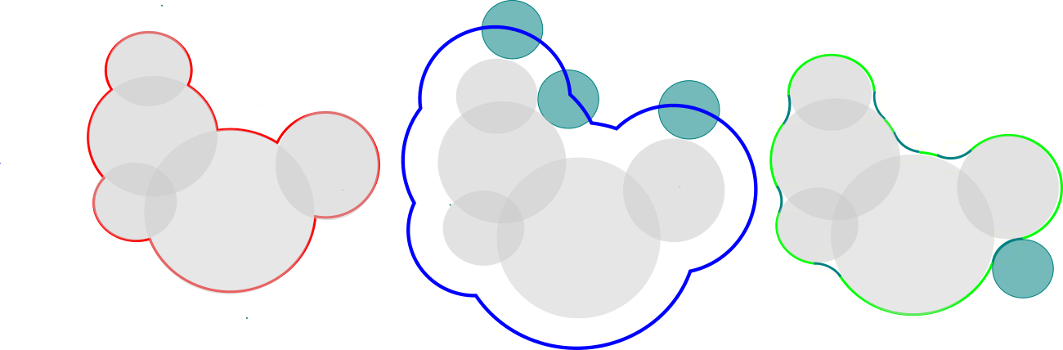
\includegraphics[width=12cm]{figure/surface.png} &
     \end{tabular}
     
     \caption{\textbf{les trois types classiques de surfaces pour une molécule} à gauche et en rouge la surface de van der waals (svdw), au centre et en bleu, la surface accessible au solvant (sa), à droite et en vert  la surface de connolly ou surface moléculaire (sm).la surface sa est l'ensemble des positions pouvant être occupées par le centre d'une sphère (figurant une molécule du solvant) roulant sur svdw.la surface sm est la plus petite enveloppe de svdw dont chaque point peut être en contact avec la sphère. } 
\label{graph:surface}
   \end{figure}
   

\subsection{modèle casa}

nous pouvons remarquer que les dipoles du solvant s'oriente , au moins pour les plus proches du soluté, selon les lignes du champ électrique crée par la protéine, voir figure \ref{graph:ecrantage}.l'idée du modèle \og coulomb accessible surface area\fg (casa)  est alors de considérer que l'effet induit par les dipoles est proportionnel à l'effet du champ électrostatique produit par la protéine qui est supposée fixe. 

on a  alors, en utilisant le modèle \texblt{SA} pour le terme non polaire:

\begin{equation}
\delta g_{solv} \approx e_{screen} + \sum_i \sigma_{t_i} a_i
\end{equation}

avec 

\begin{equation}
e_{screen} =  (\frac{1}{\epsilon} -1 )e_{coul}
\end{equation}

avec $ \epsilon $ la constante diélectrique du solvant.
ainsi, l'ecrantage est décrit par un facteur unique pour toutes les interactions électrstatiques.la simplicité de ce modèle proposé par wesson et einsenberg [212] fait de lui un modèle fréquement utilisée. cependant, il est en difficulté pour le traitement de la surface des protéines.


   \begin{figure}[t]
     \centering
     \begin{tabular}{c}
       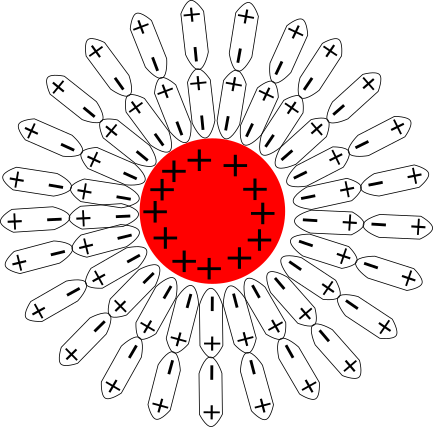
\includegraphics[width=6cm]{figure/ecrantage.png} &
     \end{tabular}
     
     \caption{\textbf{organisation des dipôles des molécules d'eau autour d'un soluté sphérique chargé négativement à sa surface}}
\label{graph:ecrantage}
   \end{figure}
   


\subsection{modèle poisson boltzmann}
la méthode de poisson boltzmann est très utilisés parce qu'elle fournit des résultats de grande précision,prend en compte l'effet ionique et toute la forme de la protéine. dans cette méthode, la protéine est supposée fixe, elle forme une cavité dans un milieu continu diélectrique qui peut est polarisé (on parle de continuum), il s'agit donc encore d'un modèle de solvant implicite.par contre les charges de la  proteine sont traitées de façon explicite par une distribution de charge. ainsi ce modèle est capable de prendre en compte l'écrantage du solvant et les interactions électrostatiques entre groupes chargés de la proteine et solvant polarisé.si le continuum est munie d'une distribution de charge $\rho$ , alors le potentiel électrostatique dans ce milieu est donnée par l'équation de poisson:

\begin{equation}
  \label{eq:poisson}
  \nabla [ \epsilon(x) \phi(x)] = - 4 \pi \rho(x)   
\end{equation}

avec $\epsilon(x)$ la constante dielectrique (ici fonction du milieu, à deux valeurs possibles) , $\phi (x)$ le potentiel électrostatique,$\nabla \phi(x)$ la divergence de $\phi$ en $x$ .

typiquement \epsilon prend des valeurs faibles , entre $1$ à $8$ pour la protéine et élévée pour le solvant, proche de $80$ pour l'eau.

l'équation de poisson-boltzmann est une extension de l'équation de poisson dans laquelle les charges d'ions mobiles sont pris en compte.la théorie de debye-hückel donne la distribution des ions comme suivant une loi de boltzmann (d'où son nom):

\begin{equation}
  \nabla [ \epsilon (x) \phi(x)] = -4 \pi ( \rho(x) - \epsilon(x) \kappa^2 \phi(x))
\end{equation}

avec $ \kappa $ le paramètre de debye-hückel qui tient compte de la concentration des ions en solution.


malheureusement, il n'existe pas , pour les protéines , de solution analytique à \ref{eq:poisson}. il faut effectué une résolution numérique. plusieurs programmes sont à la disposition de la communauté, delphi \ref{}, apbs \ref{}  qui sont basés sur la méthodes des différences finies \ref{} et des éléments finis \ref{}.

une fois l'équation résolue, le terme électrostatique de l'énergie de solvatation est donnée par:

\begin{equation}
\Delta G_{solv}^{elec} = \frac{1}{2} \int \rho(x)\phi(x)dx  
\end{equation}

Quelque soit l'approche utilisée les calculs sont couteux pour une protéine entière.



   \begin{figure}[t]
     \centering
     \begin{tabular}{c}
       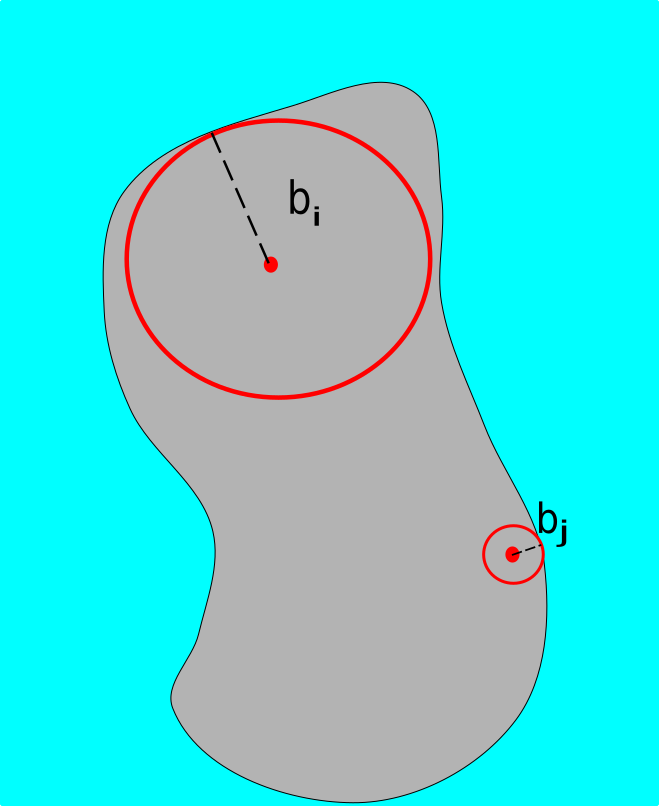
\includegraphics[width=8cm]{figure/rayon_Born.png} &
     \end{tabular}
     
     \caption{\textbf{Des rayons de Born de deux atomes dans une protéine} Le rayon de Born pour l'atome enfui est environ le rayon de la protéine, alors que le rayon de Born d'un atome à la surface est environ son rayon de Ver der Vaals.} 
\label{graph:surface}
   \end{figure}



\subsection{modèle de Born Généralisé}
\label{sub:GB}
Dans le cas d'un soluté spérique de rayon $b$ et de charge pontuelle q portée par le centre de la sphére, Born en 1930  parvient à établir des expressions analytiques des solutions de l'équation de Poisson-Boltzmann et de $ \Delta G_{solv}^{elec}$:


\begin{equation}
  \label{eq:Born}
  \Delta G_{solv}^{elec} = - \tau \frac{q^2}{2b}
\end{equation}


avec $ \tau = \frac{1}{\epsilon_p} - \frac{1}{\epsilon_s}$ , $\epsilon_p$ la constante diélectrque dela sphère et $\epsilon_s$ celle du solvant.

Partant de cette solution Still et al (1990), propose une généralisation à un ensemble d'atomes chargés formant une cavité de forme quelconque.L'objectif est alors de donner les résultats de  qualité proche de celles de PB avec un coût numérique bien inférieur.

Dans un premier temps, on évalue l'énergie libre électrostatique totale d'un ensemble de $N$ particules, de rayon $a_i$ de charge $q_i$ séparés deux à deux d'une distance $d_{ij}$ dans une milieu de constante diélectrique $\epsilon$:


\begin{equation}
  \label{eq:GB}
  G_{elec} =  E_{Coul} + \Delta G_{solv}
\end{equation}

ce qui donne;

\begin{equation}
  \label{eq:GB}
 G_{elec} =  \frac[1}{2}  \sum_{i \neq j} \frac{q_iq_j}{d_{ij}}- \frac{1}{2}  \tau \sum_i\frac{q_i^2}{\a_i}
\end{equation}

avec $ \tau = \frac{1}{\epsilon_p} - \frac{1}{\epsilon_s}$, $\epsilon_p$ la constante diélectrqiue pour les atomes et $ \epsilon_s$ celle du solvant.


L'idée consiste alors a etendre le somme sur les atomes $i$ du dernire terme en une double somme sur les paires d'atomes:


\begin{equation}
  G_{elec} = \frac{1}{2} \sum_{i \neq j} \frac{q_iq_j}{d_{ij}} - \tau \frac{1}{2} \sum_{i,j} g_{ij}
\end{equation}

avec

\begin{equation}
  \label{eq:GBg}
  g_{ij}= \tau q_iq_j (r²_{ij} + b_ib_j exp(-r²_{ij}/4b_ib_j)})^{-1/2} 
\end{equation}

avec $b_i$ et $b_j$  ,nouveaux paramètres , que l'on nomme les rayons de solvatations de l'atome $i$ et $j$.
Dans le cas où $i=j$, $g_{ij}$ est égale à deux fois l'énergie de solvatation de Born pour un ion de rayon $b_i$.
Lorsque $r_{ij}$ tend vers l'infini $g_{ij}$ la loi de Coulomb dans le solvant: $frac{q_iq_j}{\epsilon_s r_{ij}}$.

La méthode classique d'approximation des rayons de Born se fait par l'énergie libre électrostatique de l'atome $i$, dans la situation où toutes les autres particules ont une charge ramenée à zéro.Ainsi, chaque charge  de la protéine est caractérisée par sa distance au solvant.Alors, ce modèle permet le calcul de l'énergie libre de solvatation électrostatique à partir de la seule connaissance du volume de la protéine contrairement à PD qui nécessite intégration du solvant dans les calculs.
\label{NEA}

\section{l'algorithme d'exploration}

Après, un choix de l'espace d'état des conformations/séquences, après la construction d'une fonction d'énergie qui qualitie les états d'interét.Il reste, pour completer les ingrediants de bases du CPD, à choisir un algorithme d'exploration de l'espace d'état qui permet la sélection d'un sous-ensemble de séquences selon la pertinance établi par la fonction de score. Dans l'idélal,l'objectif du CPD est d'obtenir l'ensemble de séquences d'acide aminés qui sont compatibles à une structure 3D de repliment ou qui réalisent une fonction donnée.Un tel algorithme a pour grand défi de faire face à immensité de l'espace d'état. On peut classer les différentes approchent utilisées en deux groupes.

  Le premier groupe est constitué des méthodes deterministes dans lesquelles les choix effectués sont toujours soient determiné  a priori soient determiné en fonction des éléments obtenus au court de l'execution du programme qui l'implement. On trouve par exemple dans ce groupe, les méthodes exhaustives qui peuvent être appliqué à de petites espaces conformationnels ou encore les méthodes dites semi-exhaustives dans lesquels la complexité combinatoire est réduite en autorisant uniquement  certaines conformation à certain moments de l'exploration.Un classe interessante de ce groupe est consituté des algorithmes exactes qui se focalise non pas sur l'objectif du  CPD , mais sur l'obtention  de la conformation  de meilleure  énergie on parle alors de \og Global Minimum Energy Cost \fg (GMEC).
Typiquement, ces algorithmes exploitent les structures de la fonction d'énergie et de l'espace d'état.Si elle est additifs par paires de rotamères,un type particulier de méthodes est alors exploitable.Bien souvent, ces algorithmes  nécessitent un pré-calcul des énergies et le stockage de celles-ci , ce qui peut être problématique , par exemple dans les situations où le backbone est reflixe, un nombre d'état possible de la chaîne latérale vient multiplié par autant la taille de l'espace de phase. Or parmi les états qu'il faut calculer le nombre de ceux qui ne sont sans intérêt pour l'exploration de l'espace peut devenir considérable. Ce qui constitut un facteur de ralentissement . 
  
\begin{enumerate}
  Le second groupe est celui des méthodes stochastiques et/ou heuristiques. Elles ont vocation à determiner des solutions de qualité sans obtenir de garantie sur l'optimum en énergie des solutions, dans un temps d'éxecution réaliste. Elles sont non-deterministes c'est à dire qu'elles choisisent certains éléments de facon aléatoire, en pratique la \og source de hasard\fg est constituée par des générateurs de nombre pseudo-aléatoire.Elles ont l'avantage d'être utilisables sur les espaces d'états non-discretisé, par exemple [154], les rotamére peuvent varier de façon continue.Elle ne néssecite pas de connaissance a proiri sur l'espace des phases.il est souvent possible de mettre en place un systeme simple qui stocke un jeu d'énergie après une premiere utilisation, pour le réutiliser lors de futurs necessités. Par contre la convergence bien qu'elle puisse être etablie en théorie, reste en pratique difficile à cerner et n'offre pas la possibilité de reconnaitre le GMEC.Ce qui conduit au besoin de choisir une condition d'arret de l'execution sans liant direct avec ce minimum.  

\end{enumerate}

Pour rendre possible l'utilisation de plusieurs outils algoritmique , il devient nécessaire d'imposer des contraintes sur la structure de la fonction d' l'énergie. Il existe alors en CPD doit être décomposable en une energie dite propre qui rassemble les effets de la chaîne latérale et du bakbone, d'une part et une énergie d'interaction rotamère-rotamère qui se decompose comme une somme sur des interactions sur les couples de chaines latérales prises deux à deux.

on a alors la formule suivante:

\begin{equation}
E{c} = \sum_i E_i(r_i) + \sum_{i\neq j} E_{ij}(r_i,r_j)
\end{equation}


Nous présentons quelques algorithme parmis les plus utilisés.

\subsection{Algorithme du champ moyen}
Le principe de la méthode du champ moyen est le substituer l'ensembles des interactions d'un rotamère $r_0$ avec les autres rotamères par une interaction unique moyenne. Pour calculer une interaction moyenne, la probabilité de Boltzmann est utilisée de la façon suivante, on note $P(r_{i})$ la probabilité que la chaîne latérale à la position $i$ soit dans l'état rotamère $r_i$, on a:
\begin{equation}
P(r_i) =\frac{\exp(-\betaE(r_{i})})}{\sum_{l_i=1}^{N_i} \exp{-\beta E(l_i)}}
\end{equation}
avec $N_i$ le nombre total de rotamère à la position $i$ , et $\beta = \frac{1}{RT}$,  $R$ étant la constante des gas parfaits et T la température.

Si l'on ne limite au cas où une énergie d'interaction pour un résidu est la somme des interactions avec les autres positions de la chaîne, alors l'énergie d'interaction moyenne en $i$ est la somme des interactions impliquant le rotamère $r_i$ pondéré par le poids de Boltzmann de l'autre rotamère, c'est à dire

\begin{equation}
E(r_i) = \sum_{i \neq j} \sum_l_j^N_j E(r_i,l_j)P(l_j)
\end{equation}  

avec $l_j$ parcourant tous les rotamères aux positions autres que $i$.

Les formules () et (), constitue un système itératif.Ainsi, l'algorithme debute


\begin{enumerate}
\item  Etape 0 à chaque position, les rotamères sont équiprobable.
\item  Etape 1 Les énergies moyennes sont calculées grâce à la formule ().
\item  Etape 2 De nouvelles probabilités de Boltzmann sont calculées à partir des énergies moyennes precedentes   
\end{enumerate}


Les étapes 1 et 2 sont répétée jusqu'à convergence des énergies.Cette méthode garantit la convergence vers un ensemble de rotamère un plus stable à chaque position placé dans son \og environnement moyen\fg .Le temps de calculs avec cet algorithme augmente  de façon linéaire avec le nombre de résidus de la protéine.Ce qui en fait un des algorithmes les plus rapides.

\subsection{Dead-End Elimination}

Le \og Dead End Elimination\fg (DEE)  consite à éliminer des mauvais rotamères , ou des mauvaises combinaisons de rotamères qui ne peuvent pas aboutir à la combianisons de rotamère qui minimisent de façon global, l'énergie.Comme pour le champ moyen, l'énergie doit être décomposable en une energie propre et une énergie de paires.

Il y a deux critères d'élimination (Goldstein [1994]),(Desmet [1992]):

\begin{enumerate}
\item Le critère simple:
  Le rotamère $r_i$ du résidu $i$ est éliminé si la meilleure énergie (la plus faible) qu'il est possible d'obtenir pour une conformation conprenant ce rotamère est moins bonne que la pire énergie obtenue avec un rotamère $r_i'$  à la même position.
Ainsi, une expression mathématique peut être:

  avec $E(c)$, l'energie d' une séquence-conformation $c$ de l'espace d'état.

\begin{equation}
 si   min_{r_i \in C }E(C) > max_{r_i' \in C} E(C) ,alors $r_i$ est éliminé. 
\end{equation}
En utilisant l'expression  d'une fonction d'énergie décomposée par paires:

\begin{equation}
E(c) = \sum_i E_i (r_i) + \sum_{i\neq j} E_{ij} (r_i, r_j)
\end{equation}

Le critère peut s'écrire:
\begin{equation}
 si   E_i(r_i) + \sum_{j\neq i} min_{r_j} E_{ij}(r_i,r_j) > E_i(r_i') + \sum_{j\neq i}^{N} max_{r_j}E_{ij}(r_i',r_j) ,alors $r_i$ est éliminé. 
\end{equation}

avec, $N$ le nombre de positions .


\item Le critère double:
  Il exprime une condition analogue sur un couple de rotamère $(r_i,r_j)$ pour pouvoir l'éliminer, dans le sens qu'il n'est pas possible qu'il fasse partie du GMEC..Pour son expression on introduit l'énergie d'une paire $(r_i,r_j)$:


\begin{equation}

 E^{r_i,r_j} = E_i(r_i) + E_j(r_j) + Eij(r_i,r_j)  
\end{equation}

On a alors,

\begin{equation}
si E^{r_i,r_j} + \sum_{k=1}^N min_{r_k} (E_{ik}(r_i,r_k) + E_{jk}(r_j,r_k)) >  E^{r_i',r_j'} + \sum_{k=1}^N min_{r_k} (E_{ik}(r_i',r_k) + E_{jk}(r_j',r_k)) , alors la paire $r_i$,$r_j$ est éliminé.
\end{equation}
  
L'élimination d'un couple $(r_i,r_j)$, n'exclue pas pour autant la présence de $r_i$ ou de $r_j$ dans la solution optimale. 

\item le critère de Goldstein \ref{}
  Il s'agit d'une amélioration du critère simple du DEE. Il peut existe des situations dans lesquelles l'énergie avec un rotamère $r_i$  est toujours diminuée en la remplaçant par un autre rotamère $r'_i$. On peut donc l'éliminer. Or, cela n'implique pas forcement la condition du critère simple.Ce critère peut s'expirmer de la façon suivante:

\begin{equation}
si E_i^{r_i} - E_i^{r_j}+ \sum_{k=1}^N min_{r_k} (E_{ik}(r_i,r_k) + E_{jk}(r_j,r_k)) > 0, alors $r_i$ est éliminé.
\end{equation}

Voir la figure ....
  
\end{enumerate}
Au court de l'optimisation, les deux critéres peuvent être utilisé alternativement, jusqu'à qu'il n'y est plus de rotamère à éliminer.Il est alors possible d'utiliser une approche hexausitve sur l'espace d'états réduit obtenu, pour obtenir le GMEC.

Cette méthode permet dans les bons cas ( par exemple pour les petits systèmes) de converger en un temps raisonnable[26].Beaucoup de variantes du DEE [158,152] ont été proposé Pierce NA, Spriet JA, Desmet J, Mayo SL. (2000). Conformational splitting: a more powerful criterion for dead-end elimination. J Comput Chem 21: 999-1009. Notament en travaillant sur des ensembles de plus de deux rotamère.

figure figure...

\subsection{le CFN}

La méthode des réseaux de fonction de coût est issue du domaine de l'optimisation combinatoire. Il s'agît ici encore d'une méthode utilisable si la fonction d'énergie est décomposable par paires.De plus elle nécessite un pré-calcul des énergies.
Il s'agît avant tout d'une recherche de la séquence-conformation qui minimise l'énergie globale, mais qui dans certaines conditions peut également fournir un ensemble de séquence-conformation proche du GMEC.

Un réseau de fonction de coût , ou cost function network (CFN) , est défini par un triplet {X,D,C} tel que:

\begin{enumerate}
\item X un ensemble de variables à valeurs dans \mathbb{N}
\item D, un ensemble de domaines pour les variables de X
 \item C, un ensemble de fonctions, dont chaque élément porte sur un sous-ensemble S de X et donne un coût strictement positif pour chaque combinaison  de valeurs des variables de S.

\end{enumerate}  


Un problème CPD peut alors être représenté sous la forme d'un CFN, en associant chaque résidu $i$ variable d'une protéine par une variable $v_i$ du CFN, L'ensemble des rotamères possible en $i$ definissant le domaine de $v_i$.Le terme E_i représentant l'énergie \og self \fg correspond à une fonction de C tel que $S={v_i}$ et le terme E_{ij} à ne fonction de C avec $S={v_i,v_j}$.A une sequence-conformation correspond donc un valeur de D  pour chaque variable de X, on parle de solution du CFN.La recherche du minimum globale d'énergie revient alors à trouver une solution qui miminise la somme de toutes les fonctions de coût.
  
La résolution est tenté généralement par un algorithme de type  \og Depth-First Branch and Bound \fg ( ou DFBB).
les ingrédients sont les suivants:
\begin{enumerate}
\item un principe de séparation

Un ensemble des solutions peut être vu comme un sommet $S_0$ d'une arborescence sans branche.  
La séparation est l'action de partager, selon certain critère, ce sommet initial en sous-ensembles  qui devient les sommets fils de $S_0$,ce partage devant constituer une partition de l'ensemble des solutions de départ.
Le critère de séparation classique est d'énumérer les valeurs possible d'une variable $v_i$ du  CFN.A chacune des valeurs $x$ de $v_i$ on définit le sous-ensemble de $S_0$ ayant dans toutes ses solutions, $v_i$ égale à $x$.voir exemple en \ref{}. Ainso, si $v_i$ à N valeurs possible, N fils de $S_0$ sont créés.
\item un majorant
 Le majorant du problème correspond au meilleur coût connu.Il majore le GMEC.
\item un minorant d'un sommet
Le minorant correspond à une valeur que l'on sait être inférieur ou égal au coût de toute les solutions d'un sommet  
\item un principe d'évaluation
L'évaluation d'un sommet $S$, c'est déterminer un de ces minorants .Donc si un sommet est évalué et est supérieur au majorant courant,on sait qu' aucune solution de $S$ ne peut être le GMEC.La totalité du sous arbre peut être élagué ( i.e exclu de l'optimisation.  

\item une statégie de développement
La statégie de développement consiste à choisir une méthode de développement de l'arbre des solutions; C'est à dire céterminer l'ordre sur les sommets de l'arborescence dans lequel on va appliquer le critère de séparation.
Dans le DFBB, la statégie consiste à descendre dans les branches jusqu'à trouver un sous-arbre qu'il est possible d'élagué, alors l'algoritme remonte d'une branche pour redescendre dans une autre direction.Ce parcours en profondeur à l'avantage 
de limiter l'utitlisation de la mémoire, parce qu'il n'est nécessaire de conserver que la description de la branche qui a été exploirée.  
\end{enumerate}  


\begin{figure}[t]
  \centering
  \begin{tabular}{c}
    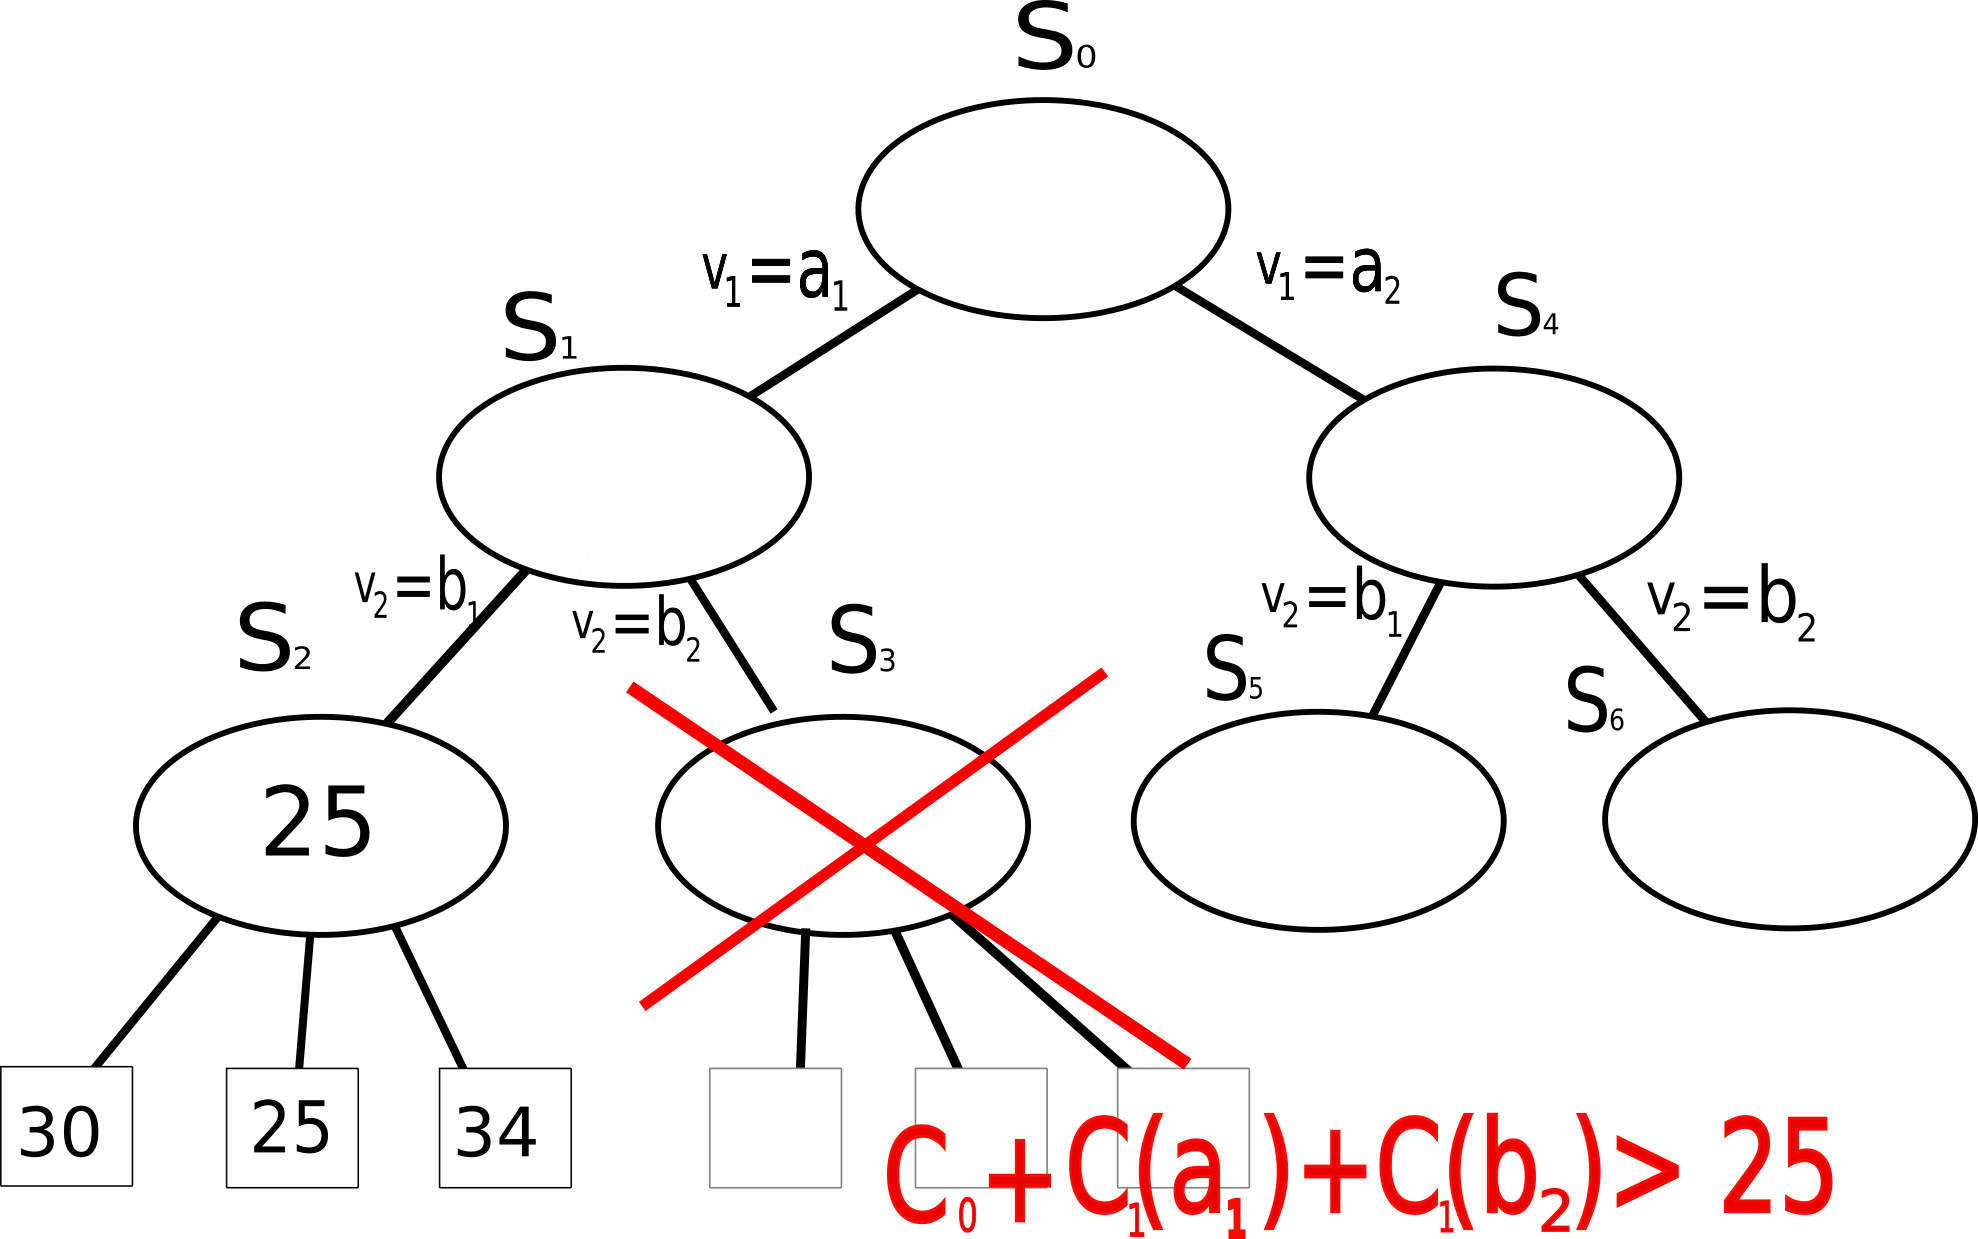
\includegraphics[width=10cm]{figure/DFBB.png} \\
  \end{tabular}
  \caption{Principe du l'algorithme du Depth-First Branch and Bound}
  \label{algo_gene}
\end{figure}



Il est alors nécesaire de trouver de bons minorants.

Equivalence Preserving Transformation

L'idée principale des cohérences locales est transformer le CFN en un CFN dans lequel le coût des affectations complètes sont identique (elles sont appelées EPT pour \og Equivalence Preserving Transformation\fg), de façon à faire apparaître de bons minorants Schiex,2000. Le principe est de déplacer les coûts entre fonctions dans le but de les attribuer aux fonctions qui portent sur une seule variable au plus (les coûts unitaires et les coûts constants) .l'avantage ici, est de pouvoir conserver les transformations dans un chemin de l'arbre de recherche tout au long de l'optimisation.Le principe est présenté sur un exemple inspiré de la thèse de Seydou Traoré.la figure {\ref ...} représente 6 CFN équivalents.Il existe deux types de transformation la première appelé projection consiste à tranféré un cout de l'ensemble des couts unaires vers le cout constant $C_0$ , c'est la transition $A\arrow B$,des coûts binaires vers le coût constant $C_0$, (transition $B\arrow C$ ) ou encore des des coût binaires vers les coûts unaires (transition $D\arrow E$). Le second type de transformation fait l'inverse, c'est à dire transfert un cout d'une fonction unaire vers les fonction bianres impliquant la même valeur de variable transition $C \arrow D$.Une telle transformation permettant une augmentation du transfert total vers $C_0$ , CFN F.



\begin{figure}[t]
  \centering
  \begin{tabular}{c}
    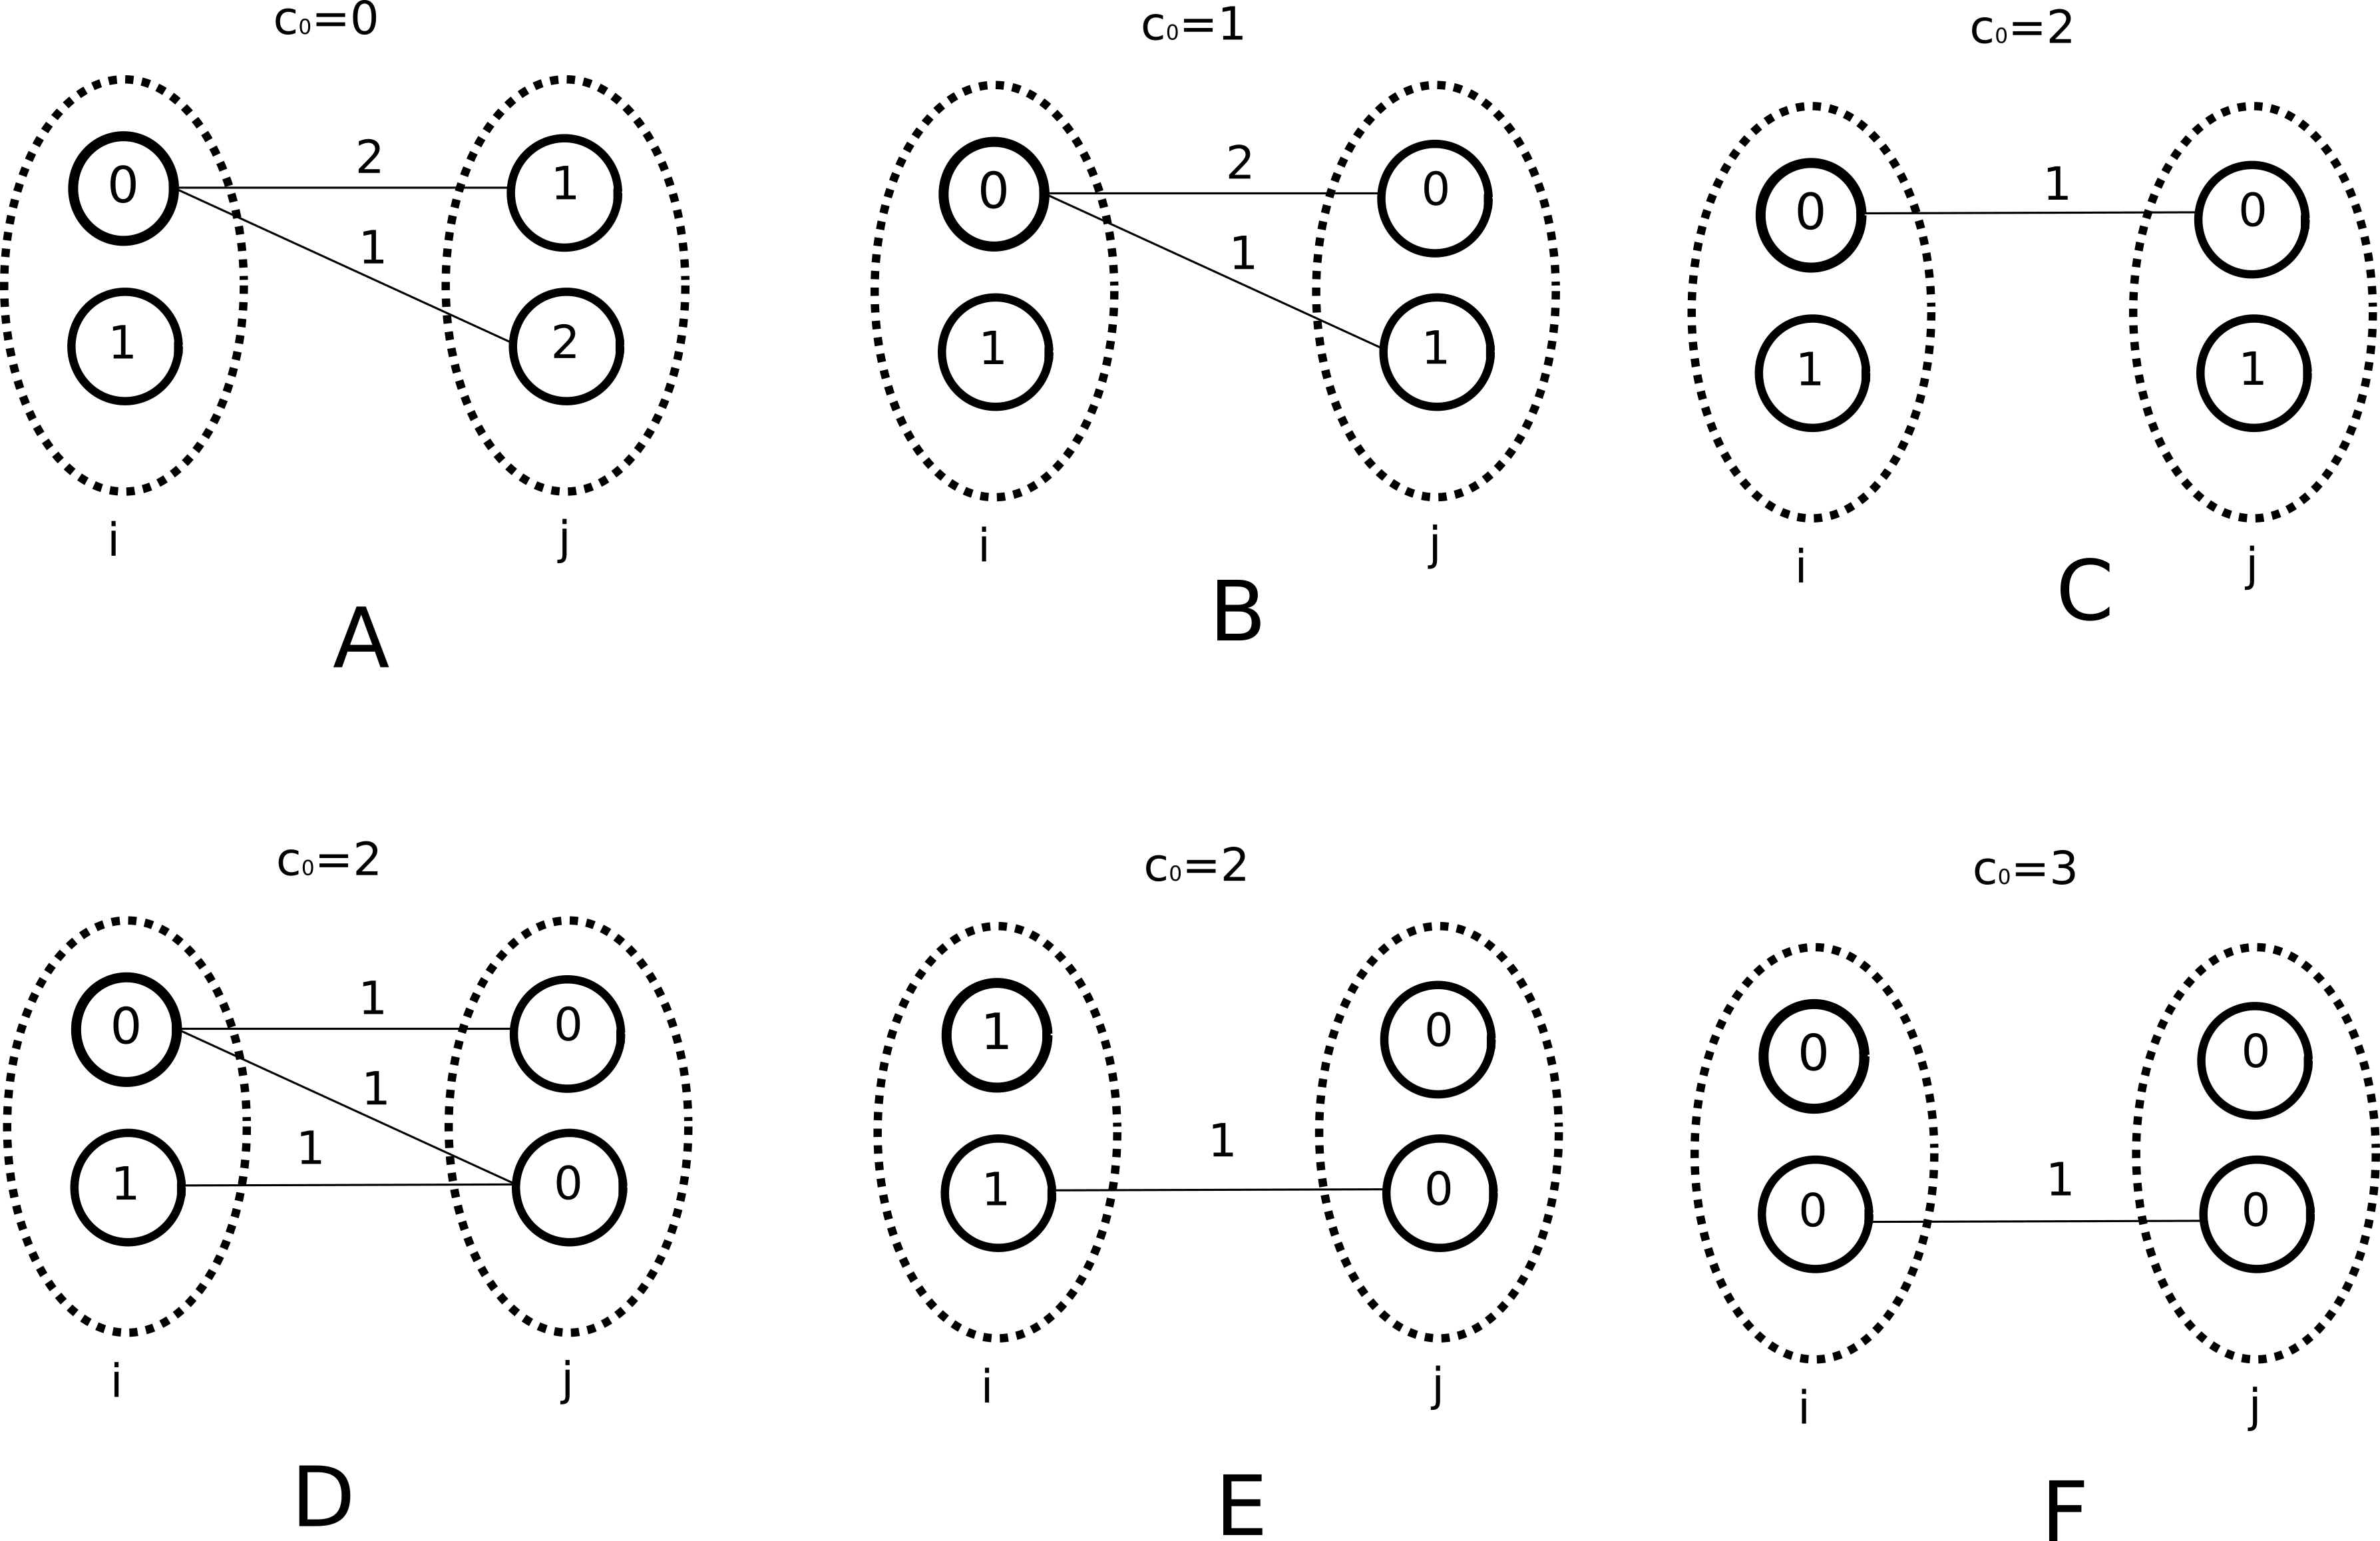
\includegraphics[width=10cm]{figure/coherences_local.png} \\
  \end{tabular}
  \caption{Exemple de transformation EPT}
  \label{EPT}
\end{figure}




Cet approche a montré sa supériorité dans le domaine du CPD , avec l'outil toulbar2 par rapport à tout un ensemble de resolveur de CFN parmi les plus réputé actuellement qui exploitent notament l'approche DEE/A* ou le backtracking \ref{}. toulbar2 en combinant FFBB,EPT et DEE a était capable de trouver le GMEC dans le plus grand nombre de problèmes proposés aux differents outils.

\subsection{l'heuristique Multistart Steepest Descent (MSD)}

En 2000,M Wernisch, Hery et Wodak partent du constat que l'espace des phases et les fonctions d'énergies qu'il est possible d'utiliser ne capture que partiellement la réalité des protéines in vivo. Ainsi, d'une part,le GMEC ne correspond par forcement à la séquence la plus stable.D'autre part, il est bien connu que des protéines homogues éloigné avec des taux d'identité à moins de $50\%$ peuvent conserver quasiment la même struture 3D, ce qui révèle l'immensité des séquences-conformations compatibles à un pli.Ainsi, l'objectif n'est plus de raisoudre une problème d'obtimisation, mais d'exiber une ensemble de séquences de basses énergie. Ils proposent alors une heuristique concut pour le CPD. Il s'agit d'un procedure simple qui a pour objectif de produire très facilement une grande quantité de séquences-conformations de basses énergie,sans se focaliser sur l'optimum.

Un cycle heuristique se déroule de la façon suivante:
Au départ, une séquence-conformation est construite en attribuant de façon aléatoire un type d'acide aminé et un rotamère à chaque position de la chaîne.Ensuite,En parcourant la séquence du début jusqu'à la fin,l'algorithme procede par des ajustements succesif à chaque position.Pour chaque position $i$ de la séquence, toutes les états possibles sont évalué, le reste de la séquence et des rotamères etant fixé.Le meilleur rotamère est alors fixé en $i$.La séquence est ainsi, ajuster par plusieurs passage successif, jusqu'à convergence de l'énergie, voir (\ref{}).

Un cycle est très rapide, ce qui permet de produite dans les cas usuels, plusieurs milliers de séquences par heures.L'utilisation mémoire hormis la gestion du stockage des énergies est quasi-nulle.Il n'impose pas que la fonction d'énergie soit pairwise, mais il s'en accommode très bien, en rendant possible l'utilisation de la mémoire par bloc des énergies impliquant une position $i$ donnée.

\begin{algorithm}
  \For{chaque cycle heuristique}{ 
    choisir une séquence-conformation $S$ aléatoirement \;
    \While{  l'énergie de $S$ est améliorée }{
      \For{  $i$ allant de la première position de $S$ jusqu'à la dernière}{
        fixer $S$ sauf à la position i \;
        determiner le meilleur rotamère possible en i  \;
        fixer $S$ en $i$ avec ce rotamère \;
      }
    }
    sauvegarder  S \;
  }
  
\end{algorithm}


\subsection{Algorithme  génétique}


Holland et ces collaborateurs introduisent une nouvelle approche inspirée des principes biologique de la sélection naturelles, avec des opérations comme les mutations, les croisements et la sélection.L'algorithme génétique a pour objectif d'obtenir un ensemble de solution proche de l'optimum en un temps raisonnable.Le shéma générale du déroulement est le suivant.Une population de séquences-conformations est générée de façon aléatoire.L'énergie de tous les membres de la population est évaluée.Un critère de sélection basée sur l'énergie est appliqué à la population, qui donc diminue.Un ensemble de mutations aléatoires et un ensemble de croisement  sont appliqués sur la nouvelle population. Donc la population augmente.Alors,une condition d'arrêt est évaluée, si elle n'est pas réalisé l'algorithme retourne à l'étape d'évaluation.
\end{enumerate}


\begin{figure}[t]
  \centering
  \begin{tabular}{c}
    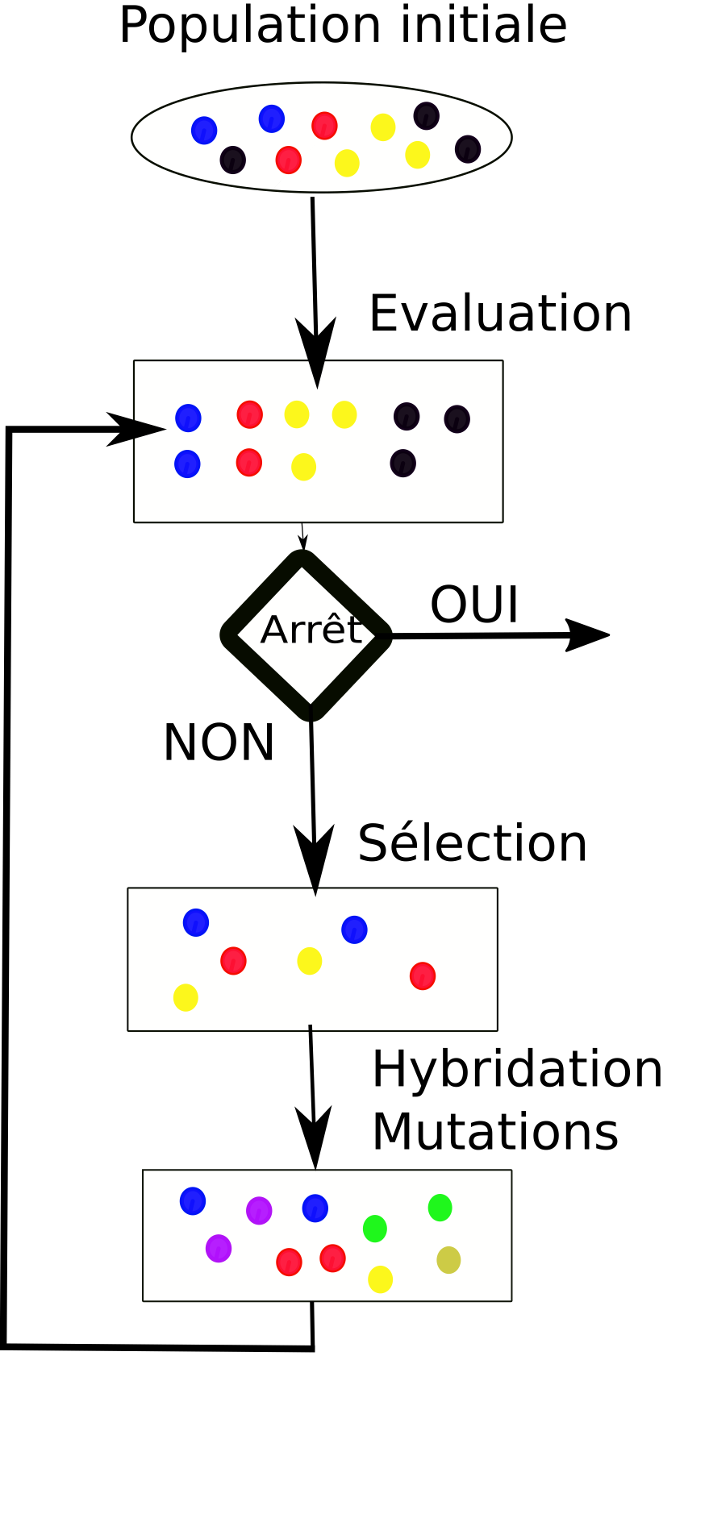
\includegraphics[width=10cm]{figure/algo_genetique.png} \\
  \end{tabular}
  \caption{L'algorithle génétique}
  \label{algo_gene}
\end{figure}


Le membre de meilleure énergie de la population tend à se reproduire le plus vite dans la population. 
Donc la valeur moyenne de l'énergie de l'ensemble des séquences-conformations converge.
On peut voir ici, que le nombre de membres de la population est un paramètre de l'algorithme.Plus ce nombre est faible plus la convergence va être rapide.A contrario, plus ce nombre est grand, plus l'exploration de l'espace d'état est meilleure.
Les atouts de l'algorithme génétique sont sa capacité à franchir des barrières énergitiques par des changements de séquences rapides via le mécanisme des croisements et sa capacité à optimiser en parallèle différents secteurs de la structure.

\subsection{Monte-Carlo}

Dans son acceptation la plus générale, un algorithme Monte-Carlo est un algorithme stochastique ( il utilise une source de hasard) qui donne approche probablement la solution exacte en un temps d'exéction déterminable a priori.Cela le distingue, parmi les algorithmes stochastiques , d'un algorithme de Las Vegas qui donne un résult
at exact dans un temps d'éxecution non deterministe , et d'un algorithme D'Atlantic City qui donne des résultats probablement correct dans un temps probablement rapide.
Parmi les algorithmes Monte-Carlo, les algorithmes Monte-Carlo par Chaînes de Markov (MCMC) ont été particulierement étudiés.
Ce ne sont pas des algorithmes d'optimisation, mais des algorithmes d'échantillonnage d'une distribution de probabilité \pi: On veut générer des éléments x_i de l'espace des phases tels que la distribution que constitue $D={x_i, i \in T \inclus \natural}$ converge vers $\pi$.

Il existe de nombreuses méthodes pour répondre à cette question, algorithme de Newton-Cotes \ref{} , algorithme du rejet \ref{} les résultats sont bons lorsque la dimension est relativement petite \ref{} tandis que les MCMC sont bien adapté dans les situations où l'espace de états est de grande dimension.Un autre avantage des algorithmes MCMC est qu'elles ne nécéssité pas la connaissance de la constante de normalisation de \pi. Cela constitué un attrait important parce que dans beaucoup de situation cette constante de normalisation est particulierement difficile à calculer.Pour ces raisons, l'échantillonnage par MCMC sont très populaire depuis plus de cinquante ans.

Dans la suite, nous donnons des conditions suffissantes pour que ce type l'algorithme converge dans le cadre d'un espace d'état $E$ fini, puis nous detaillons le plus célèbre d'entre-eux, l'algorithme de Metropolis-Hasting.

L'idée générale,est de générer un élément x_i en utilisant dans les états déjà visités uniquement x_{i-1}.Ce type de processus , où la mémoire utilisée est réduite à l'état précédent caratérise les processus de Markov.


On appelle processus stochastique, une suite de variable aléatoire {X_n}_{n\gep 0} à valeurs dans $E$.
Une chaîne de Markov est une processus stochastique tel que:

\begin{equation}
\forall n \gep 0 , \forall (i_0,i_1,...,i_{n-1},i) \in E^{n+1}, P(X_n=i|X_{n-1}=i_0,X_{n-2}=i_1,,,X_{1}=i_{n-2},X_{0}=i_{n-1},) = P(X_n=i|X_{n-1}=i_0) 
\end{equation}
Une chaîne de Markov est homogène si:

\begin{equation}
  \label{eq_homog}
\forall n \gep 0 , \forall (i,j) \in E^2, P(X_n=i|X_{n-1}=j)= P(X_{n+1}=i|X_n=j) 
\end{equation}

C'est à dire que la probabilité de transition P est indépendante de n.Dans la suite, on ne consitère que des chaînes de Markov homogènes.Et on note P(X_n=b | X_{n-1}=a) = P(b|a)


dans la suite, pour simplifier les notations, on utilise l'écriture matricielle avec

$\mu_0 =(p(X_0=i))_{i \in E},$
on a alors

$\mu_1 =\mu_0 . P$   , avec . le produit matriciel.
et

$\mu_k =\mu_0 . P^k$



Le problème revient alors à trouver une application de probabilité de transition P \muP^k -> \pi

Pour cela introduisons deux conditions supplémentaires:


Le principe de la balance détaillée:

Le principe de la balance détaillée  est un principe générale de comportement des systèmes dynamiques, il a été utilisé par Boltzmann pour la construction de la physique statistique et Cercignani et Lampis ont montré qu'il était vrai pour les gaz polyatomiques. Il peut s'exprimer de la façon suivante:

Pour un système dynamique à l'équilibre $S$ , $a$ et $b$ deux élèments de l'espace des phases, la probabilité de transition de a vers b est égale à la probabilité de transition de b vers a, ou encore: 

\begin{equation}
\forall i,j \in S
\mathcal{P}(i \rightarrow j) = \mathcal{P}(j \rightarrow i) 
\end{equation}

Pour pouvoir appliquer ce principe aux chaînes de Markov, introduisons une définition proche:

Soit q une probabilité sur E, une chaîne de Markov est dîte reversible par rapport à q si

\begin{equation}
\forall i,j \in E, q(j)P(i|j)=q(j)P(j|i)
\end{equation}

Dans ce cas, on a alors:

\begin{equation}
\forall i \in E, q.P (i) = \sum_{j \in E} q(j)P(i|j) = \sum_{j \in E} q(i)P(j|i) = q(i) \sum_{i \in E}P(j|i) = q(i)
\end{equation}

Ainsi, la probabilité q avant la transition P vaut la probabilité après, la chaîne est dîte stationnaire pour q.Il faut alors construire une chaîne de Markov reversible pour la cible \pi.

Mais cela une suffit pas, en effet même si une distribution stationnaire est connue,rien ne dit que la chaîne va entrer dedans. 

Si E est discret, une chaîne de Markov reversible est dîtes ergodique si et seulement si:

\begin{enumerate}
  \label{crit_ergo}
\item pour tous $i, j$ de l'espace d'état il existe un chemin de   $i$  vers   $j$  de probabilité non nulle. 
\item Il existe aucun x de E, tel que la chaîne revient en x périodiquement.
\item  Au court du temps,tout les états sont visités par la chaîne avec une probabilités non nulle. 
\end{enumerate}

On a alors, le résultat suivant:
Une chaîne ergodique converge vers son unique distribition stationnaire.

l'algorithme de Metropolis

Nous pouvons maintenant decrire l'algorithme de Metropolis-Hastings, L'idée initiale de Metropolis a été de construire un l'agorithme qui échantille la distribution de Boltzmann, qui donne la probabilité d'un état x_i du système en fonction son énergie et de la température:


\begin{equation}
\pi^B(i) = fraq{1}{\sum_{j \in E}E_j/kT} \exp(E_i/kT)
\end{equation}

avec $E_{x_i}$  l'énergie de $x_i$, T la température et k la constante de Boltzmann. La constante ne normalisation de la probabilté s'appelle la fonction de partition du système. Elle est particulierement difficile à calculer.

On défnit, alors la probabilité de transition P comme le produit de deux probabilités:

\begin{equation}
  \label{decomp_Metro}
P (j|i) = sel(j|i)acc(j|i)
\end{equation}

avec sel une probabilié de selectionner l'état j de E lorsque le système est dans l'état i et acc la probabilité d'accepter l'état j étant en i.Si l'on souhaite une chaîne respectant le principe de la balance détaillée par rapport à $\pi^B$, on a:

\begin{equation}
  \label{balance}
\pi^B(i)sel(j|i)acc(j|i) = \pi^B(j)sel(i|j)acc(i|j) 
\end{equation}

Si on se limite à une probabilité de selection symétrique:


\begin{equation}
\pi^B(i)acc(j|i) = \pi^B(j)acc(i|j) 
\end{equation}

ce que équivaut à

\begin{equation}
  \label{fraq_Metropolis}
fraq{acc(j|i)}{acc(i|j)} =\frac{\pi^B(j)}{\pi^B(i)} = fraq{-\exp(E_j/kT)}{\exp(E_i/kT)} = \exp(-\delta E/kT) 
\end{equation}

avec $\delta E =  E_j - E_i$.

Ainsi,le calcul de la fonction de partition est évité.

Métropolis propose alors la probabilité d'acceptation suivante:

\begin{equation}
si $\delta E >0$ alors acc(i|j) = \exp(- \delta E/kT)
sinon 
acc(i|j)=1
\end{equation}

On voit que , si $\delta E >0$ alors acc(j|i)=1 , et donc  on a bien:

\forall i,j \in E ,fraq{acc(j|i)}{acc(i|j)} = \exp(\delta E/kT)

Il suffit alors de choisir une probabilité de selection symétrique et ne violant pas \ref{crit_ergo} pour obtenir notre convergence.


Par la suite Hastings, généralise l'algorithme à une probabilité $sel()$ non symetrique avec acc() telle que:

\begin{equation}
si $\delta E >0$ alors acc(i|j) = \exp(- \delta E/kT) \fraq{sel(j|i)}{sel(i|j)}
sinon 
acc(i|j)=1
\end{equation}

Si l'on injecte cette nouvelle probabilité dans ~\ref{balance}, on a encore le respect de la balance détaillée et la convergence.


\begin{algorithm}
  Une séquence-conformation $S_0$ est choisie aléatoirement\;
  \For{ chacun des  pas $i de la trajectoire}{
    choisir une proposition  $S'_i$ à partir d'une probabilité conditionnele sel(.,S)\;
    calculer une probabilité d'acceptation acc=...\;
    \If{$acc \geq 1$}{
      $S_{i +1} = S_i'$ \;
      sauvegarder  $S_{i+1}$ \;
      }
    \Else{
      alors       $S_i +1 = S_i'$ avec une probabilité acc \;
      sauvegarder  $S_{i+1}$ \;
      \Else {
        $S_{i+1} = S_i$
      }
     }
    }
  
\end{algorithm}


Dans toute la suite, on désigne l'algorithme de Metropolis-Hastings comme l'algorithme Monte-Carlo (MC).  


Monte-Carlo avec échanges de répliques (REMC)


Une amélioration de l'algorithme de Métropolis-Hastings, connu sous le nom de \og Replica Exchange Monte-Carlo\fg a été introduite par Swendsen and Wang (Swendsen RH and Wang JS (1986) Replica Monte Carlo simulation of spin glasses Physical Review Letters 57 : 2607-2609). La méthode est également connu sont les noms \og parallel tempering\fg.L'objectif est d'accélerer la convergence en permettant au processus stochastique de visiter plusieurs zones énergitiques simultanément. Ainsi, l'algorithme couple l'exploiration dans les basins de basses énergies , importante pour la recherche des solutions optimum avec, l'exploiration dans des zones de plus hautes énergies, ce qui facilite la sortie des minimum locaux.

On considére $N$ simulations MC du système à $N$ différentes températures.Ces répliques du système sont indépendantes les-unes des autres. On note $T^m$ avec $m=1,..,N$ les differentes températures.Toutes ces temperatures sont différentes et il y a toujours exactement une replique à chaque temperature.Ainsi, nous nous placons dans un ensemble généralisé noté $E^N$, constitué des $N$-uplet $(x^1,...,x^n)$ avec les $x_i$ éléments de $E$, et $1<i<N$  indexant les répliques.On travaille alors avec une chaîne de Markov ${X_t}_{1<t}$ , avec $X_t=(x^1_t,...,x^n_t)$ sur l'espace d'état $E^N$.On ajoute alors, un nouveau type de déplacement , celui qui consiste a intervertir au temps $t$, l'état $x^i$ de la simulation à la température $T^i$ avec l'état $x^{i+1}$ à la température $T^{i+1}$.On a alors:

\begin{equation}
  \label{REMC_move}
X_{t+1}=(x_{t+1}^1,...,x_{t+1}^i,x_{t+1}^{i+1},...,x_{t+1}^n) = (x_t^1,...,x_t^i,x_t^{i+1},...,x_t^n)
\end{equation}

L'algorithme consiste alors a effectuer de façon itérative:
\begin{enumerate}
\item un ensemble de $D$ déplacements, avec $D$ une constante, de type MC 

\item puis,une tentative de déplacement de type ~\ref{REMC_move}  est effectuée.
\end{enumerate}

En effet,Pour que $X$ respecte la balance détaillée il est nécessaire d'utiliser ce nouveau mouvement dans certains conditions.Il est donc associé à une probabilité d'acceptation $acc_{swap}$ spécifique. Pour la déterminer nous reprenons la même démarche que pour le Monte-Carlo simple. Comme les repliques sont sans interactions, la distribution cible de la chaîne de Markov est égale aux produits des distributions cibles aux differentes températures:

\begin{equation}
\pi^B((x^1,...,x^n))=fraq{1}{Z}\exp(-\sum_{i=1}^N E_{x^i}/kT^i)
\end{equation}


En injectant cette expression de $\pi^B$ et ~\ref{REMC_move} dans ~\ref{frac_Metropolis} on a:


\begin{equation}
  \label{fraq_swap}

fraq{acc_{swap}(X_{t+1}|X_t}{acc_{swap}(X_t|X_{t+1})} =\frac{\pi^B(X_t)}{\pi^B(X_{t+1})} = fraq{-\exp(E_{x^j}/kT^i) -\exp(E_{x^i}/kT^j)}{-\exp(E_{x^i}/kT^i) -\exp(E_{x^j}/kT^j)} = \exp(-\delta) 
\end{equation}

avec $\delta = (\frac{1}{kT^i} -\frac{1}{kT^j})(E_{x^i} - E_{x^j})$

Ceci peut être satisfait par le critère de Metropolis:

\begin{equation}
si $\delta E >0$ alors acc_{swap} (X_{t+1}|X_t} = \exp(- \delta)
sinon 
acc_{swap} (X_{t+1}|X_t} = 1
\end{equation}

On peut alors décrire l'algorithme comme en ~\ref{REMC_algo}

\begin{algorithm}
  \label{REMC_algo}
  Lancement en parallèle de $N$ marcheurs MC aux températures ordonnées $(t_1,...,t_n)$ \;
\For{ les pas $p$ multiples d'une constante $P$}{
choisir aléatoirement $i$ compris entre $1$ et $N-1$, ce qui sélectionne les marcheurs aux températures $t_i$ et $t_{i+1}$ \;
la probabilité d'acceptation suivante est calculée acc=... \;
\If{$acc \geq 1$}{
  Les marcheurs échangent leur température \;
  \Else
      {Les marcheurs échangent leur température , avec la probabilité acc \;
      }
  }
}
\end{algorithm}


Il reste au simulateur à adapter le nombre de réplique, les températures utilisées et la fréquence des tentatives d'echange à sa problématique. La capacité de REMC à être executé sur des machines parallèles à entrainer sa grande popularité, en particulier dans le domaine de la modélisation moléculaire.Et son utilisation en physique, biologie, chimie,intelligence artificielle, etc augmente rapidement.


\section{Les programmes CPD}
\section{Les succès}

%%% Local Variables:
%%% mode: latex
%%% TeX-master: "../these"
%%% End:
